\section{Auswertung}
\label{sec:Auswertung}

Die gemessene Leerlaufspannung der Monozelle beträgt
\begin{align*}
U_0 = 1,4 \si{\volt} .
\end{align*}
\noindent Der Eingangswiderstand $R_V$ beträgt 
\begin{align*}
R_V = 10 \si{\mega\ohm} .
\end{align*}

\subsection{Bestimmung des Innenwiderstands und der Leerlaufspannung einer Monzelle}
Die gemessenen Werte für den Belastungsstrom und die Klemmenspannung sind in Tabelle (1) zu finden.

\begin{table}[H]
  \centering
  \caption{Belastungsstrom und Klemmenspannung einer Monozelle.}
  \begin{tabular}{c c}
    \toprule
     $I/mA$ & $U_K/V$  \\
    \midrule
    91,5 & 0,90\\
    70,0 & 1,10\\
    65,0 & 1,15\\
    58,0 & 1,17\\
    47,0 & 1,19\\
    41,0 & 1,23\\
    36,0 & 1,25\\
    32,0 & 1,27\\
    29,0 & 1,30\\
    25,0 & 1,32\\
  \bottomrule
  \end{tabular}
\end{table}

\noindent Mit Hilfe einer linearen Ausgleichsrechnung der Form $y = ax + b $
wird der Innenwiderstand und die Leerlaufspannung bestimmt. Die Parameter und Fehler werden mit Python berechnet.
In Abbildung (4) ist das zugehörige Diagramm dargestellt.
\begin{figure}[H]
  \centering
  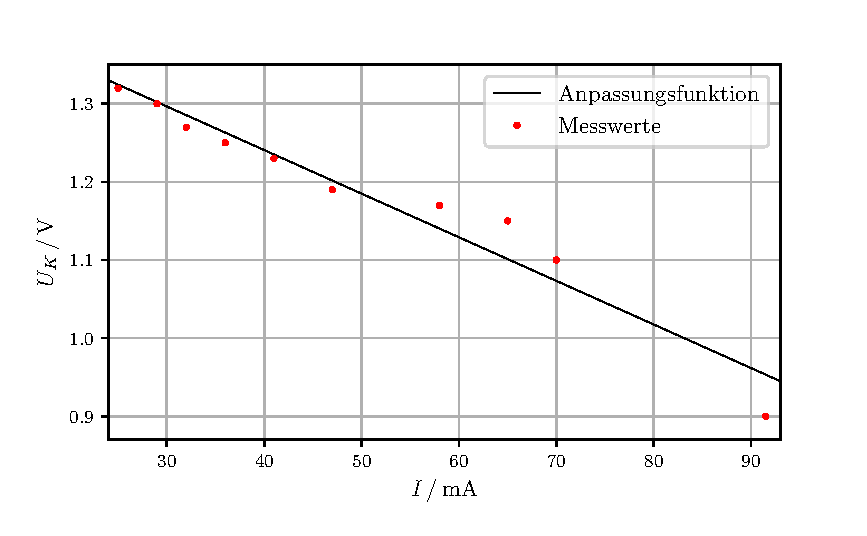
\includegraphics{plot1.pdf}
  \caption{Klemmenspannung $U_K$ der Monozelle aufgetragen gegen den Belastungsstrom $I$ in Form einer linearen Ausgleichsgeraden, und die zugehörigen Messwerte.}
  \label{fig:rechteck}
\end{figure}

\noindent Die Parameter betragen
\begin{align*}
a &= (-5,58 \pm 0,48)\Omega \\
b &= (1,46 \pm 0,03)\si{\volt} .
\end{align*}

\noindent Die Steigung $a$ ist betragsmäßig gleich dem Innenwiderstand $R_i$
\begin{align*}
R_i &= (5,58 \pm 0,48)\Omega \\
\end{align*}
\noindent und der y-Achsenabschnitt $b$ ist gleich der Leerlaufspannung $U_0$
\begin{align*}
U_0 &= (1,46 \pm 0,03)\si{\volt} ,
\end{align*} 
\noindent was sich aus Gleichung (1) ergibt.

\subsection{Bestimmung des Innenwiderstands und der Leerlaufspannung einer Monzelle mit angelegter Gegenspannung}
In Tabelle (2) sind die diesmal gemessene Spannung und Stromstärke dargestellt.

\begin{table}[H]
  \centering
  \caption{Stromstärke und Klemmenspannung einer Monozelle mit angelegter Gegenspannung.}
  \begin{tabular}{c c}
    \toprule
     $I/mA$ & $U_K/V$  \\
    \midrule
    60 & 1,77\\
    70 & 1,81\\
    80 & 1,86\\
    90 & 1,92\\
    100 & 1,98\\
    110 & 2,05\\
    120 & 2,09\\
    130 & 2,15\\
    140 & 2,20\\
    150 & 2,26\\
   
  \bottomrule
  \end{tabular}
\end{table}

\noindent Wieder wird eine lineare Regression durchgeführt, welche in Abbildung (5) aufgezeigt ist. Diesmal lauten die Parameter:
\begin{align*}
a &= R_i = (5,56 \pm 0,08)\Omega \\
b &= U_0 =  (1,43 \pm 0,01)\si{\volt} .
\end{align*}

\begin{figure}[H]
  \centering
  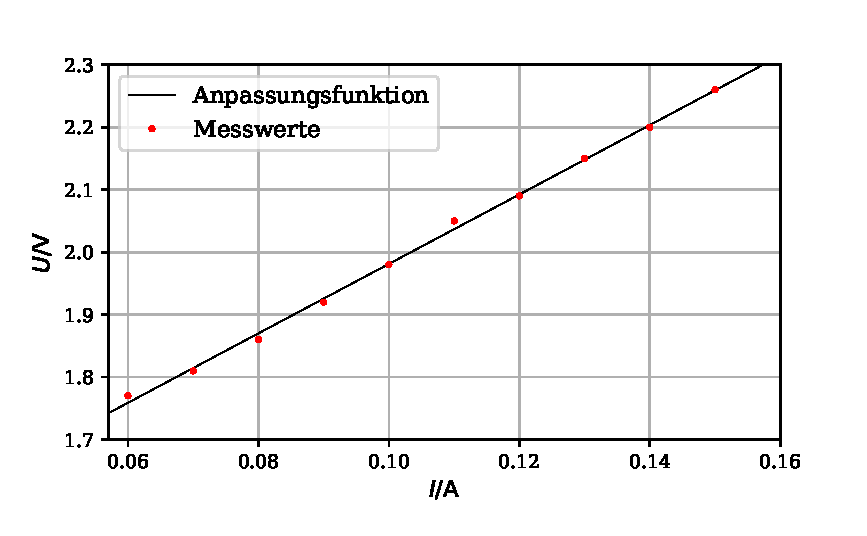
\includegraphics{plot2.pdf}
  \caption{Klemmenspannung $U_K$ der Monozelle bei angelegter Gegenspannung aufgetragen gegen den Belastungsstrom $I$ in Form einer linearen Ausgleichsgeraden, und die zugehörigen Messwerte.}
  \label{fig:rechteck}
\end{figure}

\subsection{Bestimmung des Innenwiderstands und der Leerlaufspannung einer Sinus- und Rechteckspannung}
In Tabelle  (3) sind die gemessenenen Werte für die Rechteckspannung dargelegt, und in Tabelle (4) die der Sinusspannung.
Die lineare Regression für die Rechteckspannung ist in Abbildung (6) aufgezeigt.

\begin{table}[H]
  \centering
  \caption{Belastungsstrom und Klemmenspannung bei angelegter Rechteckspannung.}
  \begin{tabular}{c c}
    \toprule
     $I/mA$ & $U/V$  \\
    \midrule
    2,2 & 0,60 \\
    2,4 & 0,59 \\
    2,7 & 0,57 \\
    2,9 & 0,56 \\
    3,3 & 0,54 \\
    3,7 & 0,52 \\
    4,2 & 0,49 \\
    4,9 & 0,46 \\
    6,2 & 0,38 \\
    8,0 & 0,28 \\
   
  \bottomrule
  \end{tabular}
\end{table}

\begin{figure}[H]
  \centering
  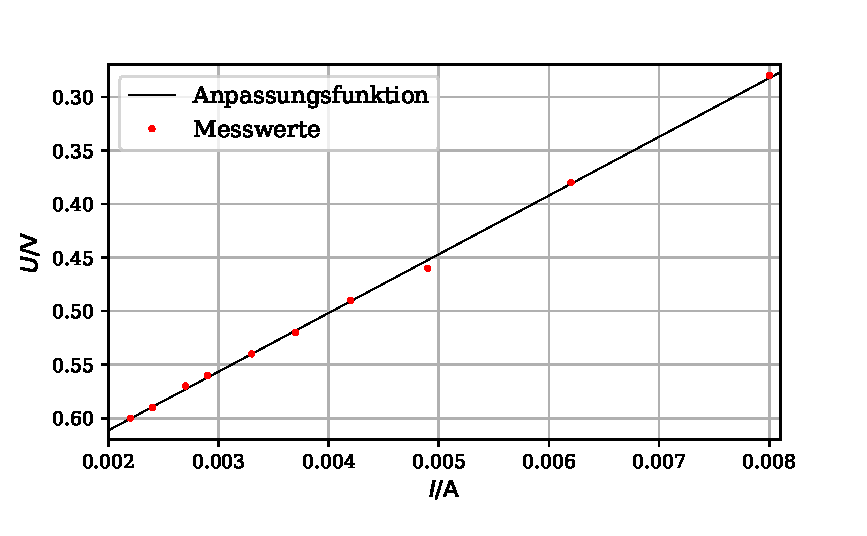
\includegraphics{plot3.pdf}
  \caption{Klemmenspannung $U$ der Rechteckspannung aufgetragen gegen den Belastungsstrom $I$ in Form einer linearen Ausgleichsgeraden, und die zugehörigen Messwerte.}
  \label{fig:rechteck}
\end{figure}

Die zugehörigen Paramter betragen:
\begin{align*}
a &= R_i = (-54,82 \pm 0,58)\Omega \\
b &= U_0 =  (0,72 \pm 0,002)\si{\volt} .
\end{align*}

Der Innenwiderstand und die Leerlaufspannung bei der Rechteckspannung lauten\begin{align*}
R_i = (54,82 \pm 0,58)\Omega \\
U_0 =  (0,72 \pm 0,002)\si{\volt} .
\end{align*}

Für die Sinusspannung wird analog verfahren; Abbildung (7) zeigt den Graphen.

\begin{table}[H]
  \centering
  \caption{Belastungsstrom und Klemmenspannung bei angelegter Sinusspannung.}
  \begin{tabular}{c c}
    \toprule
     $I/mA$ & $U/V$  \\
    \midrule
    0,50 & 2,87 \\
    0,52 & 2,87 \\
    0,58 & 2,83 \\
    0,69 & 2,75 \\
    0,79 & 2,70 \\
    0,94 & 2,60 \\
    1,10 & 2,50 \\
    1,36 & 2,33 \\
    1,77 & 2,10 \\
    2,45 & 1,63 \\
  \bottomrule
  \end{tabular}
\end{table}

\begin{figure}[H]
  \centering
  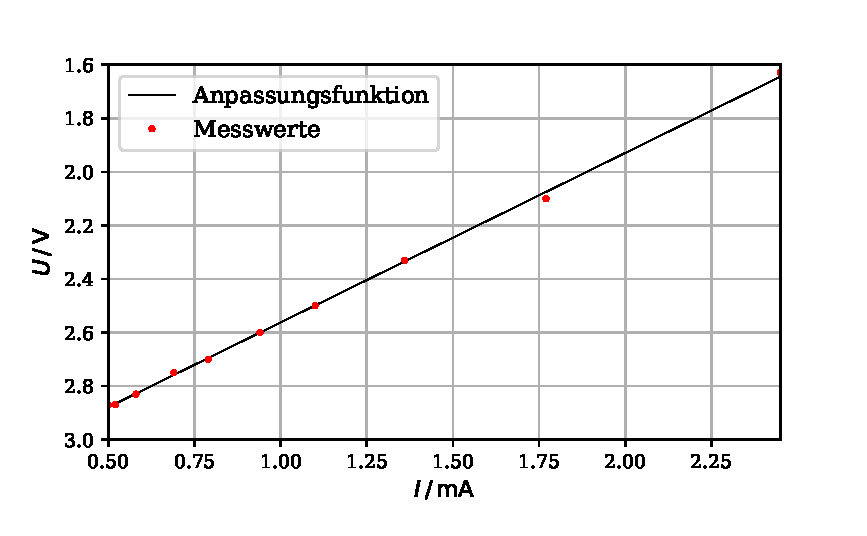
\includegraphics{plot4.pdf}
  \caption{Klemmenspannung $U$ der Sinusspannung aufgetragen gegen den Belastungsstrom $I$ in Form einer linearen Ausgleichsgeraden, und die zugehörigen Messwerte.}
  \label{fig:rechteck}
\end{figure}

\noindent Die Parameter lauten:
\begin{align*}
a &= (-632,91 \pm 6,05)\Omega \\
b &= U_0 =  (3,20 \pm 0,007)\si{\volt} .
\end{align*}
Also gilt für Innenwiderstand und Leerlaufspannung
\begin{align*}
R_i = (632,91 \pm 6,05)\Omega \\
U_0 = (3,20 \pm 0,007)\si{\volt} .
\end{align*}


\subsection{Systematische Fehler bei der Messung der Leerlaufspannung}
Den systematischen Fehler bei der Messung der Leerlaufspannung berechnet man aus Gleichung (1):

\begin{equation}
U_0 = I(R_i + R_V) = \frac{U_K}{R_V}(R_i + R_V) = U_K + \frac{U_K R_i}{R_V} .
\end{equation}
In dieser Gleichung ist $U_K$ die oben gemessene Leerlaufspannung.
Der Wert für den Innenwiderstand $R_i$ wurde in Abschnitt 1 berechnet. 
Der Fehler ist dann
\begin{align*}
\Delta U_0 &= \frac{U_K R_i}{R_V}  \\
&= (7,8 \pm 0,7) \cdot 10^{-7} \: \symup{V} .
\end{align*}
%\noindent Der Fehler von jenem Wert lässt sich mit
%\begin{align*}
%\Delta = \sqrt{(\frac{dU_0}{dR_i})^2\Delta (R_i)^2} 
%\end{align*}
%berechnen.

\noindent Schaltet man das Voltmeter hinter das reale Amperemeter, ändert sich die Spannung, da auch jenes einen Innenwiderstand $R_\text{IA}$ hat.
Der Fehler wäre dann analog
\begin{align*}
\Delta U_0 &= \frac{U_K R_i}{R_V}+\frac{U_K R_\text{IA}}{R_V} .  \\
\end{align*}

\subsection{Bestimmung der Leistung und des Belastungswiderstands}
Die Formel zur Berechnung der Leistung lautet
\begin{equation}
N = U \cdot I ,
\end{equation}
\noindent und die zur Berechnung des Belastungswiderstands
\begin{equation}
R_a = \frac{U}{I} .
\end{equation}
\noindent In Tabelle (5) sind die berechneten Werte aufgelistet.
\begin{table}[H]
  \centering
  \caption{Berechnete Leistung und berechneter Belastungswiderstand.}
  \begin{tabular}{c c}
    \toprule
    $N/$W & $R/ \symup{\Omega}$  \\
    \midrule
    0.082 & 9.836 \\
    0.077 & 15.71 \\
    0.075 & 17.69 \\
    0.068 & 20.17 \\
    0.056 & 25.32 \\
    0.050 & 30.00 \\
    0.045 & 34.72 \\
    0.041 & 39.69 \\
    0.038 & 44.83 \\
    0.033 & 52.80 \\
   
  \bottomrule
  \end{tabular}
\end{table}

\noindent Die Kurve für die Leistung wird aus den Gleichungen (1) und (2) berechnet:
\begin{align*}
I R_a &= U_0 - I R_i \\
\leftrightarrow I &= \frac{U_0}{R_a + R_i} \\
\rightarrow N &= \frac{U_0^2}{(R_a + R_i)^2}R_a
\end{align*}
\noindent Die in Tabelle (5) aufgelisteten Werte werden in Abbildung (8) dargestellt, sowie 
die Kurve $N=f(R_a)$.
\begin{figure}[H]
  \centering
  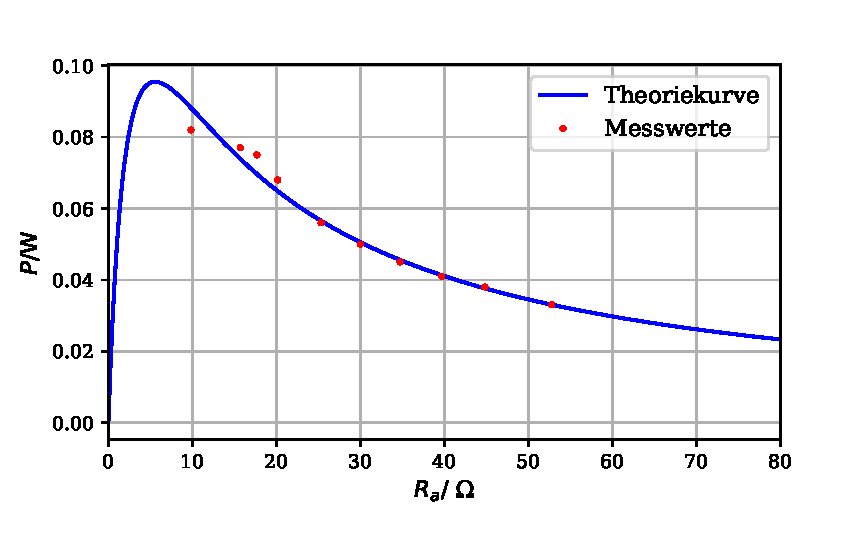
\includegraphics{plot5.pdf}
  \caption{Die Kurve der Leistung einer Monozelle und die berechneten Werte.}
\end{figure}